\documentclass{article}

\usepackage{fancyhdr}
\usepackage{extramarks}
\usepackage{amsmath}
\usepackage{amsthm}
\usepackage{amsfonts}
\usepackage{tikz}
\usepackage[plain]{algorithm}
\usepackage{algpseudocode}
\usepackage[12pt]{extsizes} %
\usepackage{enumitem}
\usepackage{multirow}
\usepackage{hyperref}

\usetikzlibrary{automata,positioning}

\topmargin=-0.45in
\evensidemargin=0in
\oddsidemargin=0in
\textwidth=6.5in
\textheight=9.0in
\headsep=0.25in

\linespread{1.1}

\pagestyle{fancy}
\lhead{\hmwkAuthorName}
\chead{\hmwkClass\  \hmwkTitle}
\rhead{\firstxmark}
\lfoot{\lastxmark}
\cfoot{\thepage}

\renewcommand\headrulewidth{0.4pt}
\renewcommand\footrulewidth{0.4pt}

\setlength\parindent{0pt}

\newcommand{\enterProblemHeader}[1]{
    \nobreak\extramarks{}{Problem \arabic{#1} continued on next page\ldots}\nobreak{}
    \nobreak\extramarks{Problem \arabic{#1} (continued)}{Problem \arabic{#1} continued on next page\ldots}\nobreak{}
}

\newcommand{\exitProblemHeader}[1]{
    \nobreak\extramarks{Problem \arabic{#1} (continued)}{Problem \arabic{#1} continued on next page\ldots}\nobreak{}
    \stepcounter{#1}
    \nobreak\extramarks{Problem \arabic{#1}}{}\nobreak{}
}

\setcounter{secnumdepth}{0}
\newcounter{partCounter}
\newcounter{homeworkProblemCounter}
\setcounter{homeworkProblemCounter}{1}
\nobreak\extramarks{prolog}{}\nobreak{}


\newenvironment{homeworkProblem}[1][-1]{
    \ifnum#1>0
        \setcounter{homeworkProblemCounter}{#1}
    \fi
    \section{Prolog \arabic{homeworkProblemCounter}}
    \setcounter{partCounter}{1}
    \enterProblemHeader{homeworkProblemCounter}
}{
    \exitProblemHeader{homeworkProblemCounter}
}

\newcommand{\hmwkTitle}{Assignment #1}
\newcommand{\hmwkDueDate}{March 9, 2021}
\newcommand{\hmwkClass}{AI}
\newcommand{\hmwkClassTime}{l.lymarenko@innopolis.university}
\newcommand{\hmwkClassInstructor}{}
\newcommand{\hmwkAuthorName}{\textbf{Lev Lymarenko}}

\title{
    \vspace{2in}
    \textmd{\textbf{\hmwkClass:\ \hmwkTitle}}\\
    \normalsize\vspace{0.1in}\small{Due\ on\ \hmwkDueDate}\\
    \vspace{0.1in}\large{\textit{\hmwkClassInstructor\ \hmwkClassTime}}
    \vspace{3in}\\\text{BS19-02}
}

\author{\hmwkAuthorName}
\date{}

\renewcommand{\part}[1]{\textbf{\large Part \Alph{partCounter}}\stepcounter{partCounter}\\}

%
% Various Helper Commands
%

% Useful for algorithms
\newcommand{\alg}[1]{\textsc{\bfseries \footnotesize #1}}

% For derivatives
\newcommand{\deriv}[1]{\frac{\mathrm{d}}{\mathrm{d}x} (#1)}

% For partial derivatives
\newcommand{\pderiv}[2]{\frac{\partial}{\partial #1} (#2)}

% Integral dx
\newcommand{\dx}{\mathrm{d}x}

% Alias for the Solution section header
\newcommand{\solution}{\textbf{\large Solution}}

% Probability commands: Expectation, Variance, Covariance, Bias
\newcommand{\E}{\mathrm{E}}
\newcommand{\Var}{\mathrm{Var}}
\newcommand{\Cov}{\mathrm{Cov}}
\newcommand{\Bias}{\mathrm{Bias}}
\newcommand{\C}{COVID }

% My commands %
\newcommand\same
 {\Leftrightarrow}

\begin{document}

\maketitle

\pagebreak
\section{PEAS}
\begin{itemize}
    \item Performance Measure - the number of steps the agent should take to reach the house
    \item Environment - 9*9 (or less) square lattice
    \item Actuator - move horizontally, vertically and diagonally
    \item Sensor - sensor to get home location, ability to perceive \C
\end{itemize}
\subsubsection{Description of the environment}
\begin{itemize}
    \item \textit{Partially Observable} since we can only perceive \C when we are nearby
    \item \textit{Deterministic} - world is fully determined by the rules, no random
    \item \textit{Single-agent} - there is no any other agents in the maze
    \item \textit{Static} - the environment does not change while an agent is acting
    \item \textit{Discrete} - there are a limited number of states of the environment
    \item \textit{Sequential} - since current move decision has consequences on future decisions
    \item \textit{Known} - designer of the agent have full knowledge of the rules of the environment
\end{itemize}

\newpage
\section{Algorithms description}
I implemented two algorithms: backtracking and A*
\subsection{Backtracking}
Backtracking solves problem recursively, considering every possible combination in order find path to home.
In order to increase performance of the algorithm, it is reasonable to introduce some optimization. For instance, on a recursion step, we can check validness of next movement, introduce maximum length of the path and do not enter already visited cells.
\subsection{A*}
As the second algorithm, I decided to choose A*.
Basically, the algorithm uses heuristic to find path. So, for every point we assign a number that shows a certain heuristic value. The logic for selecting a number may vary. In my algorithm I use the number of cells from point to the home:
\begin{verbatim}
heuristic(Point, Result) :-
    Point = Cell-_,
    home(Home),
    mooreDistance(Cell, Home, Result).
mooreDistance(X1-Y1, X2-Y2, D) :-
    D is max(abs(X1 - X2), abs(Y1 - Y2)).
\end{verbatim}

However, we should consider mask/doctor effect, so we need some modification of A*. In order to do it, I decided to introduce the meaning of covid-flag. The thing is that every cell in a maze actually represented in the algorithm twice: a cell that was entered  by actor without a mask/doctor effect and entered with a mask/doctor effect. So, technically, maze is not 2D array anymore but 3D with only two options for 3rd value: zero (no mask/doctor) and one (have mask/doctor).


\section{Comparison or two algorithms}

Actually, there is no difference between two scenarios of perceiving COVID in my algorithms:

\begin{itemize}
    \item \textbf{Backtracking} takes into account only the adjacent cells, it can not look ahead to the \C
    \item For \textbf{A*}, it is possible to consider forbidden cells from the \C in heuristic function. But it is completely not clear how to add this information to the function. Furthermore, it will not give an advantage because the actor will be less likely go the \C, which on most maps may be the wrong approach.
\end{itemize}

Consequently, we will discuss only 

\textbf{Backtracking (variant 1) compared to 2nd algorithm (variant 1)}


\subsection{Legend}
\begin{itemize}
    \item . - Free cell
    \item A - Initial actor cell
    \item M - Mask cell 
    \item D - Doctor cell
    \item C - Covid cell
    \item H - Home cell
    \item All lowercase letters is visited cells
\end{itemize}
\subsection{Maps}
In order to compare performance of two algorithms, let's construct 3 maps with different difficulty levels:
\\

\begin{verbatim}
 EASY MAP            NORMAL MAP               HARD MAP
  0 1 2 3        0 1 2 3 4 5 6 7 8        0 1 2 3 4 5 6 7 8
0 A . . M      0 A H . . M D . . .      0 A . . . . . M . D
1 . . . .      1 . . C . . . . . .      1 . . . . . . C . .
2 D . . C      2 . . . . . . . . .      2 . . . . . . . . .
3 . . C H      3 . . . . . . . . .      3 . . . . . . . . .
               4 . . C . . . . . .      4 . . . . . . . . .
               5 . . . . . . . . .      5 . . . . . . . . .
               6 . . . . . . . . .      6 . . . . . . . . .
               7 . . . . . . . . .      7 . C . . . . . . .
               8 . . . . . . . . .      8 H . . . . . . . . 
\end{verbatim}

And let's run all 3 algorithms 100 times on all 3 the maps:
\begin{center}
    

\begin{tabular}{|l|l|l|l|l|}
\hline
\multirow{2}{*}{Map\textbackslash{}Algorithm} & \multicolumn{2}{l|}{Backtracking} & \multicolumn{2}{l|}{A*} \\ \cline{2-5} 
                                              & \# of steps         & average time & \# of steps    & average time\\ \hline
Easy map                                      & 6                   &0.0345 s     & 6              &0.0205 s \\ \hline
Normal map                                    & 17                 & 78.3298 s    & 17             &0.0412 s        \\ \hline
Hard map                                      &-&too long&19&0.0857 s\\ \hline
\end{tabular}
\end{center}

So, as you can see, \textbf{backtracking} is much worse than \textbf{A*} in terms of time-consuming. Actually, A* can find path in rather big maze in a fairly reasonable time (500x500 in 16 seconds), while backtracking will try to find all possible combinations and will not be able to meet a reasonable amount of time.
\\
However, it is not fair to say that A* is better than backtracking. Prolog is not intended for implementing algorithms such as A* or Dijkstra. To achieve this goal, you have to use a lot of workarounds, creating complex data structures and turning each loop into a recursion. Thus, the implementation of a simple algorithm turns into a complex challenge. While backtracking is built into the prolog and its implementation takes several lines.

\section{Impossible to solve maps}

It is possible to solve any map without \C, so, the only option for us to create imposible map is block the path to home/mask/doctor with \C

Examples:

\\

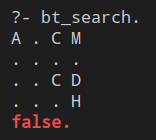
\includegraphics[scale=1.7]{impossible_map_1.png}
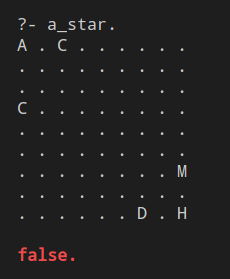
\includegraphics[scale=0.9]{impossible_map_2.png}

\\

\section{Interesting outcome/map}

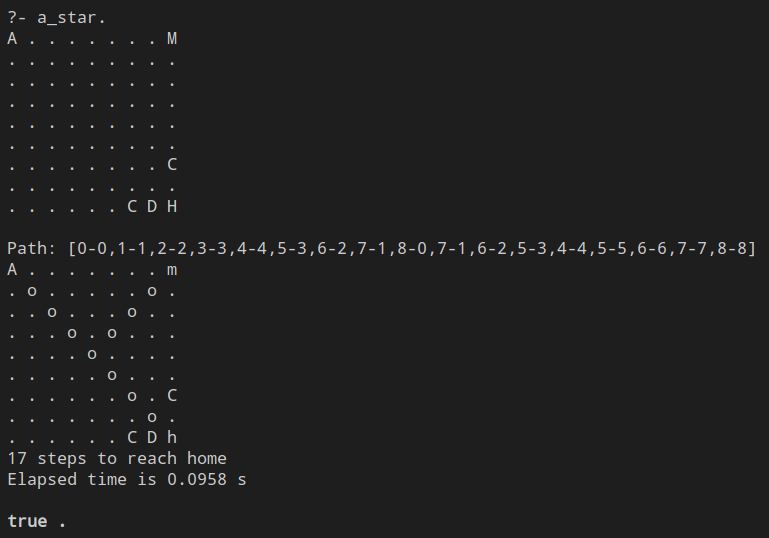
\includegraphics[scale=0.85]{interesting_map.png}

When I built this map, I expected that the solution would be a path around the perimeter of the map, however, due to the allowed diagonal movements, allowed movement in visited cells and the heuristic that the path to the home is more profitable, we get this solution!

\section{Code}

You can find the code and README file on github: \url{https://github.com/sevenzing/AI_assignment_1}
\\
Or in attached files of submission 

\end{document}
